\documentclass[11pt]{article}
%\usepackage[left=2.5cm, right=2.5cm]{geometry}  
\usepackage{amsmath}
\usepackage{amssymb}
\usepackage{mathtools}
\usepackage{bbm}
\usepackage{geometry}
\geometry{left=3.18cm,right=3.18cm,top=2.54cm,bottom=2.54cm}
\usepackage{algorithm}
\usepackage{algpseudocode}
\usepackage{algorithmicx}
\usepackage{pythonhighlight}  
\usepackage{algpseudocode}  
\usepackage{tabularx}
\usepackage{algpseudocode}
\usepackage{booktabs}
\usepackage{threeparttable}  
\usepackage{multirow}
\usepackage{subfigure}
\begin{document}
\title{Tripled Graph Convolution Network}
\date{\today}
\author{Wenjie Wu, NetID: ww2159}
\maketitle
\begin{abstract}
This project focuses on the problem of classification and content based image retrieval of high resolution remote sensing images using the notion of a novel tripled graph convolution network. The GCN model has obtained popularity in learning embedding feature for irregular domain data including graphs. Like previous studies, we conclude that GCN model is an efficient tool in remote sensing classification problem, because of the ability of GCN that could preserve the neighborhood information of the structure. Moreover, a tripled network could assess the similarity between 3 input image pair and can be trained with the contrastive loss functions. In order to test the classification ability of the proposed method, we implement the proposed embeddings for the task of classification and content based image retrieval for remote sensing data on a popular UC-Merced dataset where improved performance can be observed. The contributions of the paper are:
\begin{itemize}
	\item Introduce a novel triplet graph convolution neural network which can learn discriminative feature embeddings from high resolution remote sensing image.
	\item Build a precisely high resolution remote sensing image CBIR system based on triplet graph convolution neural network.
	\item Implement proposed method on UC Merced dataset (remote sensing images).
\end{itemize}
\end{abstract}
\section{Proposed method}
\begin{figure}
	\centering
	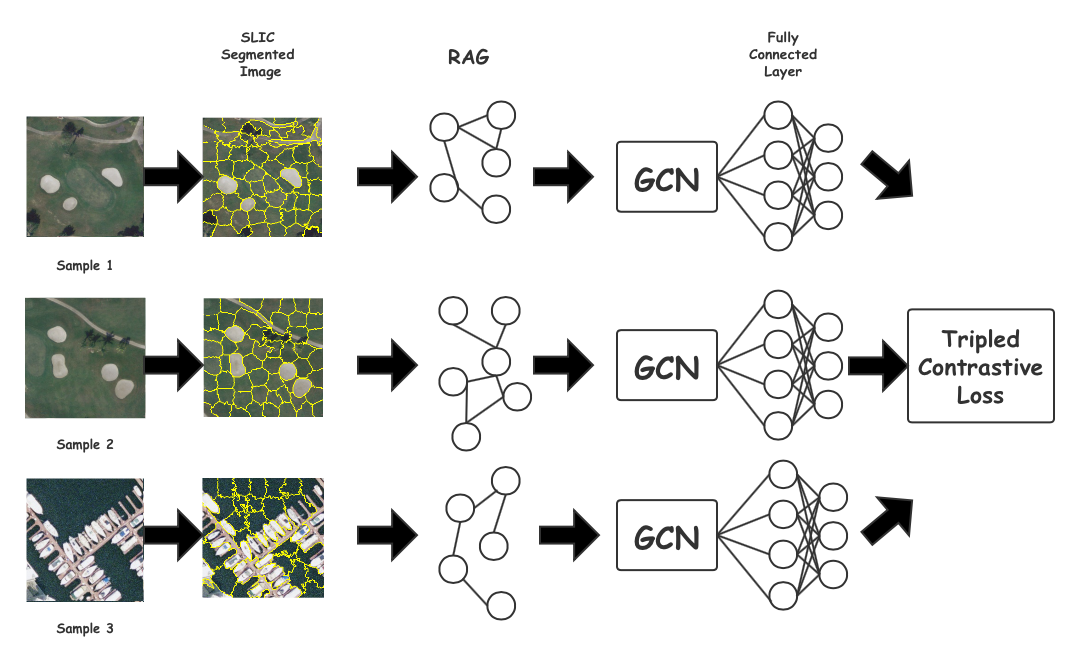
\includegraphics[width=5in]{pipeline}
	\caption{Pipeline of proposes framework}
\end{figure}
\subsection{Image segmentation}
Given an input remote sensing image dataset $X=\left\{x_1,x_2,\dots,x_n\right\}$, each $x_i$ represents an image. First, the target is to segment each remote sensing image $x_i$ into $p_i$ non-overlapping homogeneous regions $\left\{r_1^i,r_2^i,\dots,r_{p_i}^i\right\}$ using a state-of-the-art method, simple linear iterative clustering (SLIC) super-pixel. SLIC is simple to use and understand. By default, the only parameter of the algorithm is $K$, the desired number of approximately equally sized super pixels. $m$ is a constant that could be used to evaluate the relative importance between color similarity and spatial proximity. If $m$ is large, spatial proximity plays a more important role and the resulting super pixels are more solid (i.e. the super pixels have a lower area to perimeter ratio). On the other hand, When $m$ is a small number, the resulting super pixels adhere more tightly to image boundaries, but they have less regular shape and size. In the CIELAB color space, the parameter $m$ should be in the range $\left[1,40\right]$.

\floatname{algorithm}{Algorithm}  
\renewcommand{\algorithmicrequire}{\textbf{Input}}  
\renewcommand{\algorithmicensure}{\textbf{Output}}  
\begin{algorithm}  
\caption{SLIC superpixel segmentation algorithm}
\begin{algorithmic}
\Require RGB image $I$ with $N$ pixels, Paramemter $K$
\Ensure Label $l(i)$ of each pixel in image $I$
\State
\State /* Initialization */
\State Map $I$ to CIELAB color space $I_{lab}=\left[L,A,B,X,Y\right]^T$, in which $L,A,B,X,Y\in\mathbb{R}^{1\times n}$
\State Initialize cluster centers $C_k=\left[l_k,a_k,b_k,x_k,y_k\right]^T$, $k=1,2,\dots,K$ by sampling pixels at regular grid steps $S=\sqrt{N/K}$.
\For{each cluster center $C_k$}
\State Compute the gradient of each pixel in a $3\times3$ neighborhood.
\State Move cluster centers to the lowest gradient postion.
\EndFor
\For{each pixels $i$ in $I_{lab}$}
\State Set label $l(i)=-1$
\State Set distance $d(i)=\infty$
\EndFor
\State
\State /*Assignment*/
\While{error $E\leq$ threshold}
\For{each cluster center $C_k$}
\For{each pixels $i$ in $2S\times2S$ neighborhood around $C_k$}
\State compute the distance $D$
\State $=\sqrt{\left[(l_j-l_i)^2+(a_j-a_i)^2+(b_j-b_i)^2\right]+\left[\frac{(x_j-x_i)^2+(y_j-y_i)^2}{S^2}\right]m^2}$
\If{$D<d(i)$}
\State set $d(i)=D$
\State set $l(i)=k$
\EndIf
\EndFor
\EndFor
\For{each cluster center $C_k$}
\State Compute the gradient of each pixel in a $3\times3$ neighborhood.
\State Move cluster centers to the lowest gradient postion and get the new cluster centers $C_k^{new}$.
\EndFor
\State Compute residual error $E$, which is the $L_2$ norm of the locations between $C_k$ and $C_k^{new}$.
\EndWhile
\end{algorithmic}  
\end{algorithm}  

\subsection{Feature extraction}
Then we extract ad-hoc features of each region $\left\{r_1^i,r_2^i,\dots,r_{p_i}^i\right\}$ in a image from three different aspects. Shape, color and texture are really important, especially in region-based retrieval of remote sensing images \cite{chaudhuri2016region}. Eventually, for a given $j$ th region $r_i^j$ of the $i$ th image, all the following features are used to obtain the $j$ th row of the feature matrix $A_i\in\mathbb{R}^{p_i\times 359}$.

\subsubsection{Shape feature}
Shape feature is constituted with Fourier descriptors \cite{Lowe1999Object} and contour-based features: 1) Fourier descriptors could encode the shape of a two-dimensional object by doing the Fourier transform at the object's boundary, where each $(x,y)$ point on the boundary would map into a complex number $x+iy$. After such an operation, the inverse Fourier transform to recover the original shape of the object. Nevertheless, if only a few terms of the inverse have been used, the boundary would become simplified, and providing a filter to make the boundary more smooth. In our shape feature, the Fourier descriptor constitute with 4 values, which is the mean and standard deviation of the magnitude and phase of the Fourier descriptors which have been used. 2) The contour-based feature has 13 values, including extent, convex area, area, filled area, perimeter, solidity and eccentricity, equivalent diameter,  orientations, Euler number, major, and minor axes lengths and bounding box. 

\subsubsection{Color feature}
Color feature including normalized color histogram and color moments: 1) The distribution of colors in an image is called a color histogram. The normalized color histogram in our context is computed by quantizing each of the channels into 32 bins, then obtaining a color histogram vector of length 96. 2) Color moments which means moments including standard deviation, skewness, and mean separately for each color channel, ultimately resulting in 9 values per region.

\subsubsection{Texture features}
Text feature meanly constitutes with spectral histogram, entropy, local binary pattern features, and local phase quantization: 1) Spectral histogram which is calculated the same as \cite{chaudhuri2016region}, horizontal and vertical Sobel filter is effective tools and the number of filters increases to 7 and feature-length to 210, and the entropy constitutes a vector of length 3 and one for each color channel. 2) Local binary pattern features \cite{Ojala2002Multiresolution} is also a simple but efficient multi-resolution method to gray-scale. The rotation invariant texture classification based on local binary patterns, nonparametric discrimination sample, and prototype distributions results in a vector of length 8. 3) Local phase quantization features \cite{Heikkil2008Blur}, which is a new descriptor for texture classification that is especially robust to image blurring, forming a vector of length 16.

\subsection{Region Adjacency Graph}
Region Adjacency Graphs, represent adjacency of regions with a graph. In region adjacency graphs, regions in the image correspond to a node in a graph. There is an edge between each pair of adjacent regions (regions whose pixels are adjacent). For each samples, given the segmentation for the $i$ th image, our target is to construct the weighted graph representation $G_i(V_i,E_i)$, in which $V_i$ representing the node set containing $p_i$ elements and $E_i\in\mathbb{R}^{p_i\times p_i}$ is a matrix denotes the edges set. If $j\sim k$,
\begin{equation}
	E_i(r_i^j,r_i^k) = \alpha\|C_{r_i^j}-C_{r_j^k}\|_2 + \beta|\theta_{r_i^j}-\theta_{r_j^k}|
\end{equation}
Note that the $C_{r_i^j}$ denotes the centroid pixel of the $j$ th region, which could compute easily through calculating the mean value of each channel in the region, result in a 3 dimension vector in RGB image. And $\theta_{r_i^j}$ is the orientation angle, it could be computed as the edge weight of between every two nodes. It can be defined as the angle between the major axis of the ellipse and horizontal axis having the same second moment as the region. Moreover, the hyper-parameter $\alpha$ and $\beta$ are fixed empirically. Finally, the dataset $X=\left\{x_1,x_2,\dots,x_N\right\}$ could be represented as RAG (region adjacency graph) form $X=\left\{G_i(V_i,E_i),A_i\right\}_{n=1}^N$.


\subsection{Graph convolution and pooling}
\subsubsection{Convolution}
Just like a conventional CNN means to extract the most important feature from the image, a GCN utilizes several filters over the graph data, and it learns the essential vertices and edges that could help classify nodes within the graph. When it comes to the case of graphs, the convolution operation is transformed as a multiplication operation between the input vertex features $V_i$ and the adjacency matrix $H\in\mathbb{R}^{n\times n}$, which helps in preserving the spatial structure of the graph and their associated weights \cite{Petroski2017Robust}. The adjacency matrix defined as 

\begin{equation}
	H=h_0I+h_1E
\end{equation}
which only takes one-hop filter into account. $I$ represents the 0-hop or the vertex being processed and $E$ represents their adjacency neighbor. Hence, $h_0$ and $h_1$ are learnable parameters. Like a general convolution neural network, the kernel size should be equal to the number of channels. In graph circumstance, the number of the channel means the dimension of the feature of each vertex (i.e. In our work, each vertex feature is a vector in $\mathbb{R}^{1\times 359}$ which means we have 359 channels need to convolute). Moreover, the graph filter $\mathcal{H}$ should map into a higher dimension when extract more than one feature matrix. Tensor $\mathcal{H}\in\mathbb{R}^{N\times N\times359\times F}$ defined as
\begin{equation}
	\mathcal{H} = \begin{pmatrix} H_{1,1} & H_{1,2}  & \cdots &  H_{1,F}\\ 
	 H_{2,1} & H_{2,2}  & \cdots &  H_{2,F}\\
	\vdots &\vdots &&\vdots\\
	 H_{359,1} & H_{359,2}  & \cdots &  H_{359,F}\end{pmatrix}
\end{equation}
and $H_{i,j}$ is the adjacency matrix mentioned above, which is written as
\begin{equation}
	H_{i,j}=h_0^{(i,j)}I+h_1^{(i,j)}E
\end{equation}
It should be noticed that this filter helps to preserve the topology structural feature while achieving a high receptive field. So the graph convolutional operation could be written as 
\begin{equation}
	A_{conv}^{(f)}=\sum_{c=1}^{359}H_{c,f}A_{in}^{(c)}+b
\end{equation}
for $f=1,2,\dots,F$, $A_{in}^{(c)}$ denotes the $c$ col of the each feature matrix $A_i$ and $b$ is a bias.
\subsubsection{Pooling}
In GCN, convolution operation only increases the number of features of each node of the image and does not change the graph structure, but the pooling operation will change the input graph structure. The Graph Embed Pooling layer could map the input graph of any size and structure into a fixed structured output graph. To produce a pooled graph reduced to a fixed $N'$ vertices, the learnable weight matrix $\mathcal{H}_{emb}\in\mathbb{R}^{N\times N\times F\times N'}$ defined as
\begin{equation}
	\mathcal{H}_{emb} = \begin{pmatrix} H_{1,1} & H_{1,2}  & \cdots &  H_{1,N'}\\ 
	 H_{2,1} & H_{2,2}  & \cdots &  H_{2,N'}\\
	\vdots &\vdots &&\vdots\\
	 H_{F,1} & H_{F,2}  & \cdots &  H_{F,N'}\end{pmatrix}
\end{equation}
multiplied by the vertices to produce a filtered output
\begin{equation}
	A_{emb}^{(n')}=\sum_{f=1}^{F}H_{f,n'}A_{conv}^{(f)}+b
\end{equation}
In which, $A_{emb}^{(n')}$ is the $n'$ col of the embed feature matrix $A_{emb}$, $A_{conv}^{(f)}$ is the aforementioned convolutional feature and $b$ is a bias. Note that in graph embed pooling, not only the adjacency matrix but also the vertices are transformed
\begin{equation}
\begin{aligned}
	A_{emb}^*&=\sigma(A_{emb})\\
	A_{pool}&=A_{emb}^{*T}A_{conv}\\
	E_{pool}&=A_{emb}^{*T}E_{in}A_{emb}^{*}
\end{aligned}
\end{equation}
In which, $E_{in}$ is the edge weight matrix of the input region adjacent graph. $\sigma(\cdot)$ is the softmax function. The softmax function is also called softargmax or the normalized exponential function. Softmax can be understood as the generalization of logistic regression classifiers facing multi-classification problems. The function takes the $K$ real vector as input and outputs, which is a probability distribution consisting of the probability of $K$ proportional to the exponent of $K$. Among these components, output vector can be interpreted as the probability that the result is each category. Furthermore, a larger input component should correspond to a greater probability. Softmax is commonly used in neural networks to map the unstandardized output of the network to the probability distribution on the predicted output category. The standard (unit) softmax function $\sigma:\mathbb{R}^{K}\rightarrow \mathbb {R}^{K}$ is defined by the formula
\begin{equation}
	\sigma(\mathbf{z})_i=\frac{e^{z_i}}{\sum_{j=1}^Ke^{z_j}}
\end{equation}
for $i = 1,2,\dots,K$ and $\mathbf{z}=(z_1,z_2,\dots,z_K)\in\mathbb{R}^K$.
\subsection{Triplet Network}
In order to learn a more differentiable feature space, a triplet network is used. Triplet network is first introduced by \cite{Hoffer2015Deep}, the author inspired by Siamese network is comprised of 3 instances of the same feed forward network which uses the same parameters. In such model a contrastive loss over the metric induced by the representation is used to train the triplet network to distinguish three samples. Three samples are selected from two classes in each forward propagation process. We denote 3 inputs as $x$, $x^+$ and $x^-$, in which $x^+$ and $x^-$ must come from different class and $x$ is not strictly required generate from which class in those two classes. A contrastive loss favours a small distance between pairs of examples labeled as similar, and large distances for pairs labeled dissimilar. In \cite{Hoffer2015Deep}, the authors mention that triplet network works out the problem that the features learned by siamese network provide sub-par results when used as features for classification. Moreover, siamese networks are also very sensitive to calibration which means the notion of similarity vs dissimilarity requires context. However, triplet network does not need such calibration. In their experiments, they have experienced hands on the difficulty in using Siamese networks. For the best of our knowledge, this is the first time that proposed graph convolution structure triplet network. The embedded layer before the last layer will be the vector
\begin{equation}
	TripletNet(x,x^-,x^+)= \begin{pmatrix} \|Net(x)-Net(x^-)\|^2\\ 
	 \|Net(x)-Net(x^+)\|^2\end{pmatrix}\in\mathbb{R}^2_+
\end{equation}
in which $Net(\cdot)$ is a fully connected network. So that the loss function is 
\begin{equation}
	Loss(d_+,d_-)=\|(d_+,d_--1)\|_2^2=const\cdot d_+^2
\end{equation}
where
\begin{equation}
	d_+=\frac{e^{\|Net(x)-Net(x^+)\|_2}}{e^{\|Net(x)-Net(x^+)\|_2}+e^{\|Net(x)-Net(x^-)\|_2}}
\end{equation}
and
\begin{equation}
	d_+=\frac{e^{\|Net(x)-Net(x^-)\|_2}}{e^{\|Net(x)-Net(x^+)\|_2}+e^{\|Net(x)-Net(x^-)\|_2}}
\end{equation}
We denote that $Loss(d_+,d_-)\rightarrow0$, if $\frac{\|Net(x)-Net(x^+)\|}{\|Net(x)-Net(x^-)\|}\rightarrow0$.
\section{Result}
In this part, we set up a benchmark experiment, the dataset we used is UC Merced, a high resolution remote sensing dataset which is brought out by \cite{Chaudhuri2018Multilabel}. In the dataset, there are 21 class (denseresidential, forest, freeway, baseballdiamond, beach, mediumresidential, golfcourse, harbor, intersection,  airplane, mobilehomepark, overpass, parkinglot, agricultural, buildings, chaparral, river, runway, sparseresidential, storagetanks, tenniscourt) land use image. And there are 100 RGB images which measures $256\times 256$ pixels for each class. The images were extracted from large images from the USGS National Map Urban Area Imagery collection and labeled manually for various urban areas around the country. The pixel resolution of this public domain imagery is 1 foot. We use general CNN (Alex Net), and RNN as our baseline methods and the architecture of the those two nets is given in table \ref{location}, in which $nF$ is a convolution layer with $n$ filter, $P/2$ is a max-pooling $/2$ layer and 2FC is a fully connected layer with 2 hidden layer. All models have a FC-21 layer and a softmax loss layer. From the result, we could tell that GCN outperforms other methods, and Tripled structure helps GCN to learn a more discriminate feature space. Also the loss of GCN converges more quickly than other method and AUC box Plot indicates that Tripled GCN and GCN are more efficient classier towards high resolution remote sensing classification problem.

\begin{table}[!t]  \caption{Detail of Benchmark Experiment}
\centering
\label{location}
\begin{tabular}{lll}  
\toprule   
Model & Architecture & Precision\\ 
\midrule   
Tripled GCN  &128F-P/2-64F-P/2-2FC-21&99.87\%\\
GCN  &128F-P/2-64F-P/2-2FC-21&97.32\%\\
CNN  &128F-P/2-64F-P/2-2FC-21&95.19\%\\
RNN &LSTM&83.26\%\\
\bottomrule  
\end{tabular}
\end{table}
\begin{figure}[H]
	\centering
	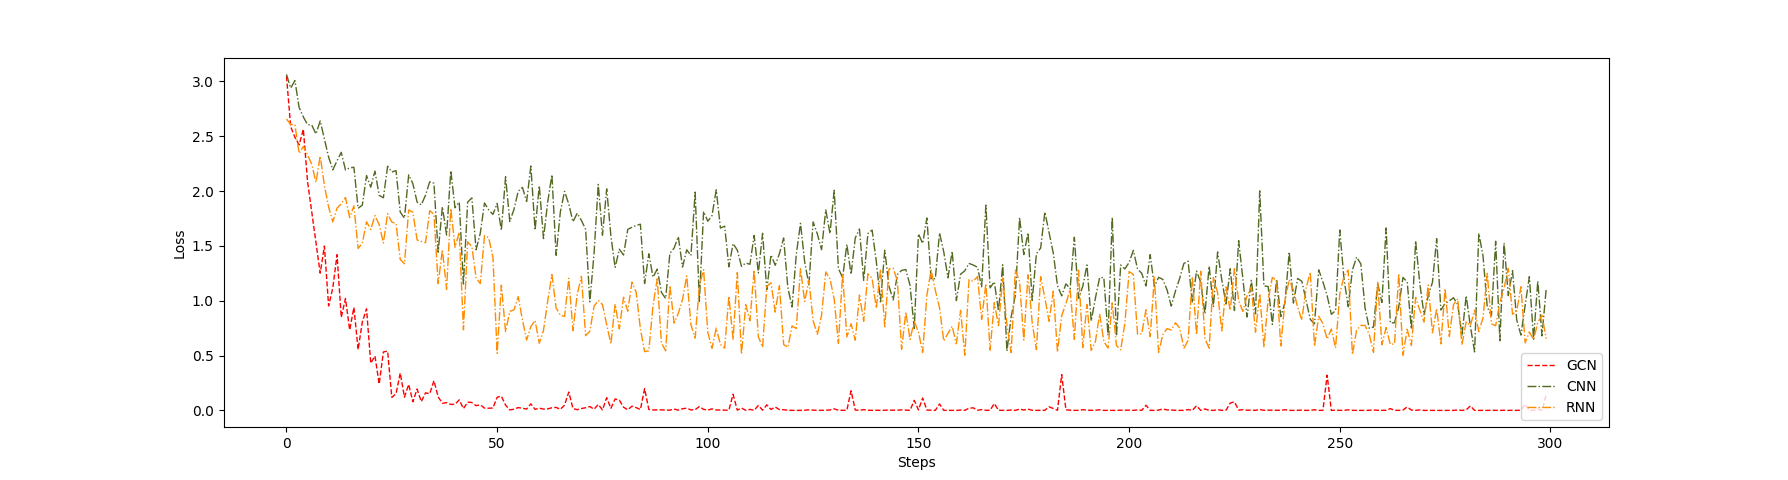
\includegraphics[width=5.2in]{Loss}
	\caption{Loss of Benchmark Experiment}
\end{figure}
\begin{figure}[H]
	\centering
	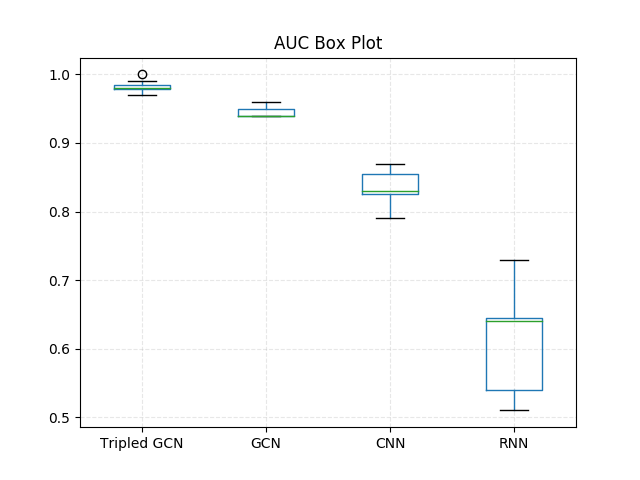
\includegraphics[width=5.2in]{box.png}
	\caption{AUC Box Plot of each method}
\end{figure}
Moreover, the content based image retrieval ability is evaluated. We choose the feature before the final softmax layer as the feature of an image, which means when the training process already been done, an in-query image would follow the pipeline 128F-P/2-64F-P/2-2FC and the obtain a feature vector $V\in\mathbb{R}^{256}$. Then the $L_2$ distance is calculated between the retrieval image and all the image in the database. Finally, an KNN algorithm is used to image retrieval (i.e. if $k=3$ those three image which has the closest distance with the in-query image would be identified).
\begin{figure}[H]
\centering
\subfigure[In-query image]{
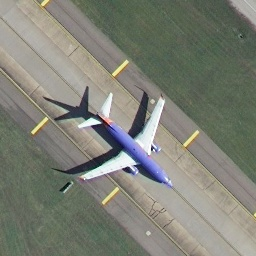
\includegraphics[width=2.7cm]{airplane10.jpeg}
}
\quad
\subfigure[Retrieval 1]{
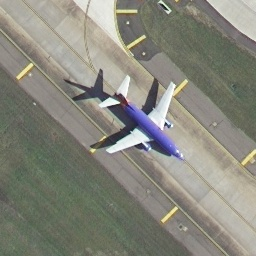
\includegraphics[width=2.7cm]{airplane19.jpeg}
}
\quad
\subfigure[Retrieval 2]{
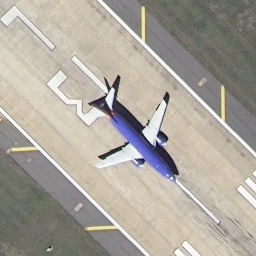
\includegraphics[width=2.7cm]{airplane8}
}


\subfigure[In-query image]{
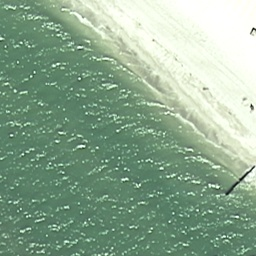
\includegraphics[width=2.7cm]{beach14}
}
\quad
\subfigure[Retrieval 1]{
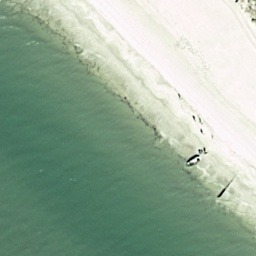
\includegraphics[width=2.7cm]{beach19}
}
\quad
\subfigure[Retrieval 2]{
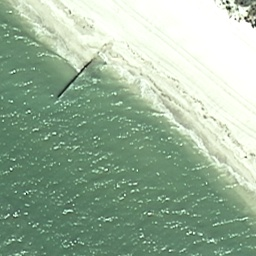
\includegraphics[width=2.7cm]{beach6}
}

\caption{Image Retrieval}
\label{heatmap}
\end{figure}

\section{Conclusions}
Many types of graph data are heterogeneous and cannot be processed using traditional spectral convolutional filtering techniques such as high-resolution remote sensing images. The GCN architecture helps us preserve the neighborhood information of the structure and offers the same breakthrough benefits currently only afforded to homogeneous data. Similar to traditional CNN architectures, Graph-CNNs operate directly in the spatial domain to generate semantically rich features. Moreover, tripled GCN is even more efficient and powerful to learn a discriminative embedding space for designing a remote sensing classifier or CBIR system. The experiment result indicates the efficiency of the proposed method. The future work may involve extending the flexibility and applications of GCN or tripled GCN method.
\newpage
\bibliographystyle{unsrt}
\bibliography{biblo}
\end{document}